\title{Teaching Literary Theories Handout}
\author{
        Ms. Holloway\\
        ENG4U1\\
        Sean Kernitsman
        }
\date{\today}

\documentclass[11pt, twocolumn]{article}
\usepackage[margin=0.5in]{geometry}
\usepackage{multicol}
\usepackage{lipsum}
\usepackage[english]{babel}
\usepackage{graphicx}


\begin{document}

\begin{twocolumn}
\maketitle
\section{Introduction}
Literary Criticism is a particular way of reading a text to see it from a different perspective. It encourages the reader to critically evaluate the meaning of the text from that perspective.
This handout presents various literary theories and criticisms.
The theories are explained in simple words and examples are provided for every theory.
% \paragraph{}


\section{Reader Response}

A reader response critic analyzes the reader's role in the production of work.
The reader creates his personal meaning of the text based on their real-world experiences.
The theory denies the possibility that works are universal, but instead, groups of people with common beliefs and opinions should interpret the text in a similar way, also known as an Interpretive Community.

The theory presents two types of readers:
\begin{enumerate}
        \item \textbf{Implied Reader}- The reader who responds to the text in a specific way.
        \item \textbf{Actual Reader}- The reader who responds based on their personal experiences in the world.
\end{enumerate}

The reader-response theory is especially useful when there are gaps in the plot for the reader to fill in and when considering the fact that people's interpretations change over time.

A reader response critic should analyze a text by considering the following:
\begin{enumerate}
        \item Identify how the reader was supposed to feel when a certain event happened.
        \item How does one's personal experience might change the anticipated meaning of the work?
\end{enumerate}

\pagebreak
\section{Marxism}
Marxism is a literary criticism that focuses on the differences between classes of society.
Those differences are in the economic and status level. Carl Marx divides society to three different levels:
\begin{enumerate}
        \item \textbf{Aristocracy}- This category is the traditional kings and queens. They have power from possessing land and rule the other categories. For example, Queen Elizabeth II.
        \item \textbf{Bourgeoise}- The bourgeoise is the working call of society. The social order is dominated by capitalism. They control the means of production. E.g.: The owner of Apple Inc.
        \item \textbf{Proletariat}- The lowest-ranked working class. The proletariat is industrial workers who seel their labour to live. They do not have any production methods. They are considered to be the lowest economic class. For example, everyone who works an ordinary 9-5.
\end{enumerate}
The lens focuses on the power dynamics between the classes and how they operate together.
A Marxist critic would identify the class of each character and how it affects their beliefs, actions and characteristics.
The base of the society is the methods of production of products and services, where the superstructure is the values generated from the base.

% \pagebreak
\section{Feminism}
The feminism criticism is concerned with the way in which women are presented in literature and other production methods of society.
This lens tries to prove how our society is dominated by males. This is also referred to as a \textbf{Patriarchy}. On the other hand, \textbf{Gynocentrism} is a society where women are dominating.
The criticism is concerned with women’s rights, equal gender representation and the way women are portrayed in literacy.
When analyzing a text from a feminist perspective, you would want to analyze the following questions:
\begin{enumerate}
        \item In the text, do women economically, politically or socially oppressed by the patriarchal ideology?
        \item How are the relationships between men and women?
        \item Does the text reinforces the ideology of patriarchy?
\end{enumerate}
Outside of literature, you could also apply the text's representation of women in the current world. Especially the three waves of feminism.
In brief, the first wave (late 1700s-early 1900's) highlights the inequalities between the sexes.
The second wave (early 1960s-late 1970s) works on building on more equal working conditions. In this time the National Organization for Women (NOW) formed.
The third wave (early 1990s-present) is about resisting the perceived essentialist ideologies and the marginalized populations' experiences.

\section{Postcolonial}

The postcolonial theory deals with the literature of colonization or colonized peoples. There are two sides of the coin, the colonized and the colonizer. The colonized are the people subjected to the ways of the colonizers.
The colonizer is a country, nation or group of people who establish political or economical control over the native people. It is common that the colonizer established hegemony (dominance) with either force or with benefits and advantages that the colonized did not have before.
The colonized could read in three different ways to the colonizer:
\begin{enumerate}
        \item \textbf{Hybridization} – The cultures mix together well (British and Indian)
        \item \textbf{Mimicry} - The colonized accepts the ways of the colonizer and gives up its previous culture.
        \item \textbf{Diaspora} - The colonizer has great power and dispose of (displace or put an end to) people who go against their beliefs.
\end{enumerate}
If at a certain point the colonizer leaves, the society would never be the same as it was before colonization.
Application to the real world- Eurocentrism is the belief that the “European” way is the right way.
Know colonized nations include the United States, Africa and South Asia.

Important questions to consider while postcolonial analyzing: \\
\begin{enumerate}
        \item Who are the colonized and colonizers? What is their power dynamics between them?
        \item How do the power dynamics affect the culture, religion and identity of the society?
        \item Does the colonizer offer the population anything for smooth colonialism?
\end{enumerate}

\section{Mythological (Archetypal)}

Mythological criticism in literature consists of the following three steps:
\begin{enumerate}
        \item Identify repeating patterns in the literature (character types, themes, plots and symbols).
        \item Identify how those repeating patterns function in the work.
        \item Assert that they shape our roles in society and literature.
\end{enumerate}
Those collective patterns are known as archetypes. Carl Jung theorized that "mankind possesses a "collective unconscious" that contains these archetypes and that is common to all of humanity".
For an example of characters, plots, themes and symbols:
\begin{itemize}
        \item \textbf{The Hero}: Associated with light. Represents society’s current ideals. The hero is faced many obstacles but manages to overcome them.
        \item \textbf{The Mother}: Always take care of her children. She could sacrifice herself for the security and safety of her children.\\
        \item \textbf{Hero vs. Villain}: Protagonist vs Antagonist. The hero usually wins at the end.
        \item \textbf{People vs. Nature}: The (usually unforeseen) forces of nature make big harm to the environment and mankind. In the end, human beings usually survive.\\
        \item \textbf{Nemesis}: People are punished or rewarded as they deserve. It usually based on good or evil actions.
        \item \textbf{Fulfillment}: A character finally comes to accept its destiny. It usually takes a long time for the character to come to a realization.\\
        \item \textbf{Water}: Represents birth and death resurrection, purification, redemption, fertility and growth.
        \item \textbf{Garden}: Paradise, fertility and innocence.
\end{itemize}

\pagebreak
\section{Psychoanalysis- Jung}

Like the Mythological theory, Psychoanalysis also focuses on the collective unconscious, but besides that, there is also the consciousness which is what is currently we thinking or aware of. This includes thoughts, feelings and desires.
Also, the unconsciousness is what we are not aware we know. It shapes who we are and how we personally behave, believe and think on a general level.

The theory explains that archetypes are different for every single person and individuation is the process where personal and collective unconscious is balanced together in harmony.
It is where the person must accept all of the different personality parts of themselves
However, they are usually not balanced, so there are four different archetypes to help in the journey:
\begin{enumerate}
        \item \textbf{The Persona}: It is a mask we put on which portrayed a different person than what we truly think of ourselves.
        \item \textbf{The Shadow}: It is the dark and hidden part of our personality. It is unconsciously hidden and refers to our evil self.
        \item \textbf{The Anima}: The inner feminine part of the male personality or a man’s image of a woman
        \item \textbf{The Animus}: An inner masculine part of the female personality or a woman’s image of a man.
        \item \textbf{The Self}: Gives a sense of harmony. Associated with religion and spiritual beliefs.
\end{enumerate}

A psychoanalytic critic would identify the characters persona, shadow, anima(mus) and the self. Then, identify if the character reaches individuation. If not, what stands in its way?

\section{Psychoanalysis- Freud}
The Freudian Psychoanalysis looks at the author's and character's psychology. It considers their motivations and how it affects their actions and psyche.
The human psyche consists of three parts:
\begin{enumerate}
        \item \textbf{The Id}: The part of ourselves that required instant gratification as fast as possible. The id does not operate logically or conscience. But rather, based on emotions and self-pleasure.
        \item \textbf{The Superego}: The personality part which makes a decision based on the conscience. It follows moral and societal code, laws and principles.
        \item \textbf{The Ego}: The ego balances the two extrema, the id and superego. It finds the golden mean between satisfaction and kindness. It uses logic, reasoning and knows what personality part to prioritize at a given situation.
\end{enumerate}

The theory also brings the idea of the preconscious- the memory part which could be recalled instantly without much effort. In addition, the unconscious also stores the instincts, fears and selfish motives.
As seen in Fig. \ref{fig:iceberg}, Freud presents a model of the psyche in sync with the different consciousnesses.

\begin{figure}[h!]
        \centering
        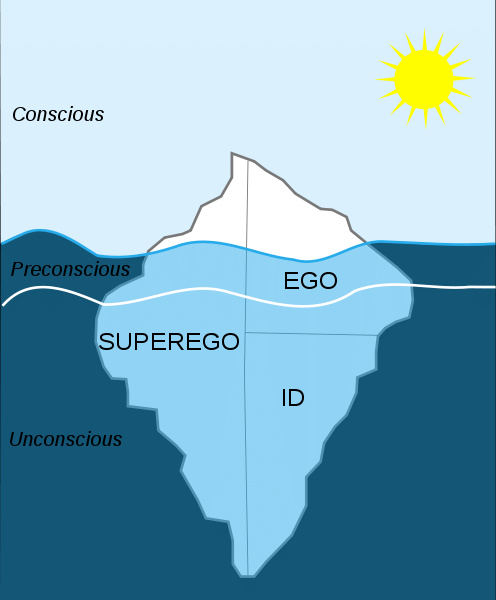
\includegraphics[width=0.2\textwidth]{assets/freud_iceberg.png}
        \caption{\textsf{The iceberd model suggested by Freud}}
        \label{fig:iceberg}
\end{figure}

Freud also suggests three defence mechanisms that deffer us from reality.
\begin{itemize}
        \item \textbf{Denial}: When faced with uncomfortable information, the mind rejects it.
        \item \textbf{Repression}: When the unconscious mind pushes away the memory or feeling away from the consciousness as it is too painful to deal with.
        \item \textbf{Displacement}: When one can not deal with pain so the unconscious mind searches for alternatives.
\end{itemize}

Freud also suggests the Freudian Drives sub theory. He believed that much human behaviour is motivated by sexuality.
\begin{itemize}
        \item \textbf{Oedipus Complex}- A boy's unconscious rivalry with his father for the love of his mother.
        \item \textbf{Elektra Complex}- A girl’s unconscious rivalry with her mother for the love of her father
\end{itemize}

A psychoanalytic critic would consider the followings:
\begin{itemize}
        \item Identify symbols in the text (such as yhonic, phallic, movement from society, evil deeds are performed, strong sexual urges)
        \item Analyze how those symbols aid in explaining the meaning of the text.
        \item How does the psyche of a character constructed? Is there a particular personality part that dominates the psyche? If so, what and why happens to the character?
\end{itemize}

\end{twocolumn}
% \lipsum
\end{document}
